\documentclass[handout]{plt}
%Use dspdfviewer program to view the presentation with notes
%\usepackage{pgfpages}
%\setbeameroption{show notes}
%\setbeameroption{show notes on second screen=right}

\title{The Lambda Calculus}
\author{Stephen A. Edwards}
\institute{Columbia University}
\date{Fall 2018}
\titlegraphic{%
  \hbox to 5pc{\hskip -1pc%
  \hbox{%
    \vbox{%
      \hbox{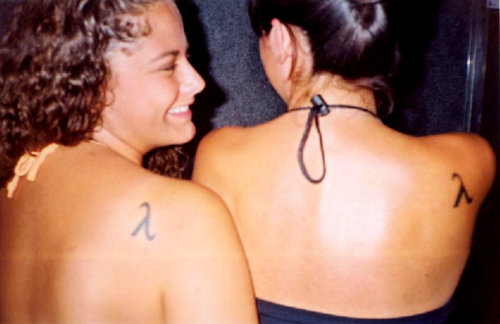
\includegraphics[height=4pc]{lambda-twins.jpg}%
        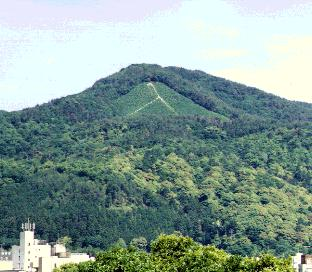
\includegraphics[height=4pc]{mount-lambda.jpg}}%
      \hbox{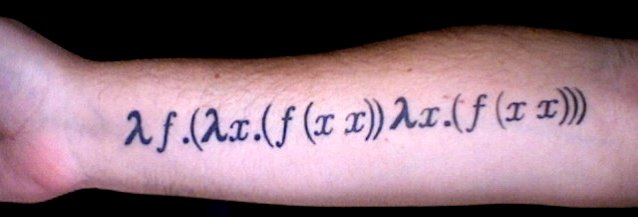
\includegraphics[height=3.6pc]{y-combinator.jpg}}%
    }%
    \hbox{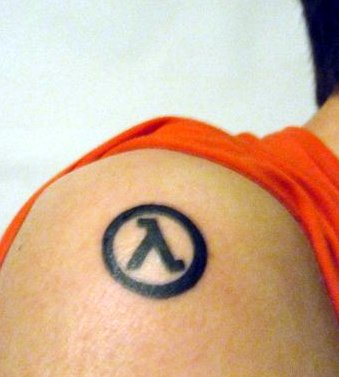
\includegraphics[height=7.6pc]{Lambda-Tattoo.jpg}}%
    \hbox{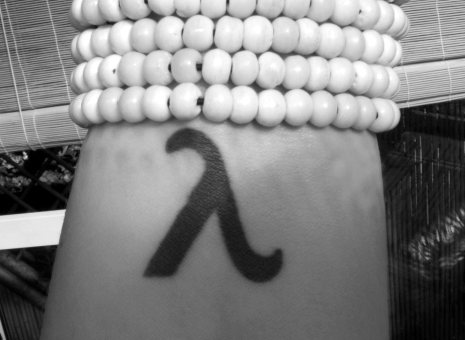
\includegraphics[height=7.6pc]{lambda-wrist.jpg}}%
    }}}

\begin{document}

\NoHyper
\maketitle

\pagenumbering{arabic}
\begin{frame}[fragile=singleslide]{Lambda Expressions}

Function application written in prefix form.  ``Add four and five'' is

\begin{lcalc}
(+ 4 5)
\end{lcalc}

Evaluation: select a \emph{redex} and evaluate it:

\begin{lcalc}
(+ (* 5 6) (* 8 3)) & \rightarrow & (+ 30 (* 8 3)) \\
& \rightarrow & (+ 30 24) \\
& \rightarrow & 54
\end{lcalc}

Often more than one way to proceed:

\begin{lcalc}
(+ (* 5 6) (* 8 3)) & \rightarrow & (+ (* 5 6) 24) \\
& \rightarrow & (+ 30 24) \\
& \rightarrow & 54
\end{lcalc}

\footnotesize
Simon Peyton Jones, \emph{The Implementation of Functional Programming
  Languages}, Prentice-Hall, 1987.

\note{
\begin{enumerate}
\item The lambda calculus is a functional language in its purest form.
\item Terms in the calculus are called
      \emph{lambda expressions} which are similar to expressions in
      Ocaml or other functional languages.
\item One category of lambda expression is function application,
      written in prefix notation. (Function comes before arguments)
\item Evaluate an expression by REDUCTION: find a reducible expression
      (or \emph{redex}) and evaluate it. A redex is basically a lambda
      expression that can be simplified.
\item In this example, we could evaluate our lambda expression in one
      of two ways. 
\end{enumerate}
}



\end{frame}

\begin{frame}[fragile=singleslide]
  \frametitlelogo{Function Application and Currying}{0.2\textwidth}{curry-powder-can.jpg}

Function application is written as juxtaposition:

\begin{lcalc}
f x
\end{lcalc}

Every function has exactly one argument.  Multiple-argument functions,
e.g., $+$, are represented by \emph{currying}, named after Haskell
Brooks Curry (1900--1982).  So,

\begin{lcalc}
(+ x)
\end{lcalc}

is the function that adds $x$ to its argument.

Function application associates left-to-right:

\begin{lcalc}
(+ 3 4) & = & ((+ 3) 4) \\
  & \rightarrow & 7 \\
\end{lcalc}

\note{
  \begin{enumerate}
  \item Unlike in Ocaml, all function application is written as
  juxtaposition (can't write 2 + 3).
  \item Furthermore, every function in the lambda calculus only has a
  single argument. Capture multi-arg functions via \emph{currying} --
  a multi-arg function becomes a sequence of single-arg function
  applications. 
  \item So (plus x) is a single-arg function that adds x to its
  argument.
  \item We can determine how a multi-argument function is curried by
  relying on associativity -- func. app associates l-to-r, so here we
  are applying a function that adds 3 to its argument to the constant
  4, evaluating to 7.
  \item TRANSITION: So we know we can apply functions in the labmda
  calculus. But if we could only use simple arithmetic this wouldn't
  be a universal language. We need to be able to create new functions!
  \end{enumerate}
}

\end{frame}

\begin{frame}[fragile=singleslide]{Lambda Abstraction}

The only other thing in the lambda calculus is \emph{lambda
  abstraction}: a notation for defining unnamed functions.

\begin{lcalc}
(\lambda{x} . + x 1)
\end{lcalc}

\[
\begin{array}{l*{7}{@{\ }c}@{\ }l}
( & \lambda & x & . & + & x & & 1 & ) \\
  & \uparrow & \uparrow & \uparrow & \uparrow & \uparrow & & \uparrow \\
 & \textsl{That function of} & x & \textsl{that} & \textsl{adds} & x &
  \textsl{to} & 1 \\
\end{array}
\]

Replace the $\lambda$ with \textbf{fun} and the dot with an arrow to
get a lambda expression in Ocaml:

\begin{center}
\begin{ocaml}
fun x -> (+) x 1
\end{ocaml}
\end{center}

\note{
  \begin{enumerate}
  \item Fittingly, the only other type of lambda expression in the
  calculus is a \emph{lambda abstraction}, which lets us define
  unnamed functions.
  \item Always start with a lambda followed by a name for the
  function's argument (always exactly one due to currying), then a dot to
  separate the argument from the function's body.
  \item READ OUT LAMBDA EXPRESSION
  \item Basically the \emph{fun} operator in ocaml (fun n -> n+1)
  \end{enumerate}
}

\end{frame}

\begin{frame}{The Syntax of the Lambda Calculus}

\begin{center}
\shadowstart
\begin{tabular}{lcl}
\textit{expr} & ::= &
\textit{expr} \textit{expr} \\
& $|$ & $\lambda$ \textit{variable} . \textit{expr} \\
& $|$ & \textit{constant} \\
& $|$ & \textit{variable} \\

& $|$ & (\textit{expr}) \\
\end{tabular}
\shadowend
\end{center}

Constants are numbers and built-in functions;\\
variables are identifiers.

Function application binds more tightly than $\lambda$:

\begin{center}
\shadowstart
$\lambda x . f g x = \lambda x .\big((f g) x\big)$
\shadowend
\end{center}

\note{
  \begin{enumerate}
  \item We can now define the full syntax for the lambda calculus.
  \item GO OVER EACH TERM.
  \item Mention that we don't actually need constants; we'll see how
  to capture them with lambda abstractions later.
  \item Note that application binds more tightly than lambda
  $\rightarrow$ basically, imagine parentheses around an abstraction's
  body.
  \end{enumerate}
}

\end{frame}

\begin{frame}[fragile=singleslide]{Beta-Reduction}

Evaluation of a lambda abstraction---\emph{beta-reduction}---is just
substitution:

\begin{lcalc}
(\lambda{x} . + x 1) 4 & \rightarrow & (+ 4 1) \\
  & \rightarrow & 5 \\
\end{lcalc}

The argument may appear more than once

\begin{lcalc}
(\lambda{x} . + x x) 4 & \rightarrow & (+ 4 4) \\
& \rightarrow & 8 
\end{lcalc}

or not at all

\begin{lcalc}
(\lambda{x} . 3) 5 \rightarrow 3
\end{lcalc}

\end{frame}

\note{
  \begin{enumerate}
  \item Given an abstraction applied to an argument, we evaluate it
  via \emph{beta-reduction} $\rightarrow$ intuitively, simple substitution.
  \item The \emph{x} is replaced with the argument 4 wherever it's
  found in the lambda's body. Then evaluate the primitive addition.
  \item GO OVER TWO OTHER MINI-EXAMPLES (note that if variable isn't
  used, argument just ``disappears'')
  \end{enumerate}
}

\begin{frame}[fragile=singleslide]{Beta-Reduction}

Fussy, but mechanical.  Extra parentheses may help.

\begin{lcalc}
(\lambda{x} . \lambda{y} . + x y) 3 4 &
  \arraycolsep=0pt
  \begin{array}[t]{cccclrr}
= & \Biggl(&\biggl(\lambda{x} . & \Bigl(\lambda{y} . & \bigl((+ x) y\bigr)\Bigr)\biggr)& 3\Biggr)& 4 \\
\rightarrow & \Biggl(&  & \lambda{y} . & \bigl((+ 3) y\bigr) & \Biggr) & 4 \\
\rightarrow & &  & & \bigl((+ 3) 4\bigr) &  & \\
\rightarrow & &  & & 7 &  &
  \end{array}
\end{lcalc}

Functions may be arguments

\begin{lcalc}
(\lambda{f} . f 3) (\lambda{x} . + x 1) & \rightarrow &
(\lambda{x} . +  x 1) 3 \\
& \rightarrow & (+ 3 1) \\
& \rightarrow & 4 \\
\end{lcalc}

\note{
  \begin{enumerate}
  \item As long as you follow the simple substitution rule, you can
  evaluate any expression in the lambda calculus!
  \item Add extra parens to make things less ambiguous (after each dot
  up to the next enclosing paren; make left-associativity of function
  application explicit). 
  \item GO THROUGH EXAMPLE 1 -- Look for a redex and evaluate it
  (explain why you have to reduce 3 before 4).
  \item Since an abstraction is itself a lambda expression, we can
  pass it as an argument to another abstraction; substituted in the
  same way.
  \item GO THROUGH EXAMPLE 2
  \item We need one more concept to describe beta-reduction formally:
  free vs. bound variables.
  \end{enumerate}
}

\end{frame}

\begin{frame}[fragile=singleslide]{Free and Bound Variables}

\begin{lcalc}
(\lambda{x} . + x y) 4
\end{lcalc}

Here, $x$ is like a function argument but $y$ is like a global
variable.

Technically, $x$ \emph{occurs bound} and $y$ \emph{occurs free} in

\begin{lcalc}
(\lambda{x} . + x y)
\end{lcalc}

However, both $x$ and $y$ occur free in

\begin{lcalc}
(+ x y)
\end{lcalc}

\note{
  \begin{enumerate}
  \item READ LITTLE EXAMPLE
  \item \emph{x} occurs bound because it's named as the enclosing
  function's parameter.  
  \item \emph{y} occurs free because it wasn't bound by this lambda.
  \item Both are free in the last expression because neither are bound
  by a lambda.
  \item ANY QUESTIONS ABOUT BOUND Vs. FREE?
  \end{enumerate}
}

\end{frame}

\begin{frame}[fragile=singleslide]{Beta-Reduction More Formally}

\begin{lcalc}
(\lambda{x} . E) F & \rightarrow_{\beta} & E'
\end{lcalc}

where $E'$ is obtained from $E$ by replacing every instance of $x$
that appears free in $E$ with $F$.

The definition of free and bound mean variables have scopes.  Only the
rightmost $x$ appears free in

\begin{lcalc}
(\lambda{x} . + (- x 1)) x 3
\end{lcalc}

so

\begin{lcalc}
(\lambda{x} . (\lambda{x} . + (- x 1)) x 3) 9 & \rightarrow &
(\lambda x . + (- x 1)) 9 3 \\
& \rightarrow & + (- 9 1) 3 \\
& \rightarrow & + 8 3 \\
& \rightarrow & 11
\end{lcalc}

\note{
  \begin{enumerate}
  \item With this notion, we can formally define beta-reduction with
  this formula (GO OVER FORMULA WITH TEXT BELOW)
  \item Trick: cover $\lambda{x}$ with your hand, then replace any
  free \emph{x}'s in E with F. HOWEVER, there may be \emph{x}s that
  are bound by sub-expressions as in this next example.
  \item This means we have scope in the lambda calculus!
  \item GO OVER BOTH EXAMPLES
  \end{enumerate}
}

\end{frame}

\begin{frame}[fragile=singleslide]{Another Example}

\begin{lcalc}
\Bigr(\lambda{x} . \lambda{y} . + x \bigl((\lambda{x} . - x 3) y\bigr)\Bigr) 5 6 &
\rightarrow & \Bigr(\lambda{y} . + 5 \bigl((\lambda{x} . - x 3) y\bigr)\Bigr) 6 \\
& \rightarrow & + 5 \bigl((\lambda{x} . - x 3) 6\bigr) \\
& \rightarrow & + 5 (- 6 3) \\
& \rightarrow & + 5 3 \\
& \rightarrow & 8 \\
\end{lcalc}

\note{
  \begin{enumerate}
  \item WALK THROUGH EXAMPLE 
  \item ANY QUESTIONS ON BETA-REDUCTION IN GENERAL?
  \item There are 3 operations other than beta-reduction that you can
  perform on lambda expressions.
  \end{enumerate}
}

\end{frame}

\begin{frame}[fragile=singleslide]{Alpha-Conversion}

One way to confuse yourself less is to do $\alpha$-conversion:
renaming a $\lambda$ argument and its bound variables.

Formal parameters are only names: they are correct if they are
consistent.

\begin{lcalc}
(\lambda{x} . (\lambda{x} . + (- x 1)) x 3) 9 & \leftrightarrow &
(\lambda{x} . (\lambda{y} . + (- y 1)) x 3) 9 \\
& \rightarrow & ((\lambda{y} . + (- y 1)) 9 3) \\
& \rightarrow & (+ (- 9 1) 3) \\
& \rightarrow & (+ 8 3) \\
& \rightarrow & 11
\end{lcalc}

You've probably done this before in C or Java:

\begin{minipage}{0.3\textwidth}
\shadowstart
\begin{lstlisting}[language=C]
int add(int x, int y)
{
  return x + y;
}
\end{lstlisting}
\shadowend
\end{minipage}
\hskip 2pc
$\leftrightarrow$
\hskip 2pc
\begin{minipage}{0.3\textwidth}
\shadowstart
\begin{lstlisting}[language=C]
int add(int a, int b)
{
  return a + b;
}
\end{lstlisting}
\shadowend
\end{minipage}

\note{
  \begin{enumerate}
  \item The first is alpha-conversion, which can help make some of the
  earlier examples less confusing.
  \item Alpha rename the inner expression's \emph{x} to \emph{y} to
  make things clearer. Unlike beta reduction, alpha-conversion leaves
  the ``meaning'' of an expression unchanged.
  \item We do stuff like this all the time in programming languages.
  \end{enumerate}
}

\end{frame}

\begin{frame}[fragile=singleslide]{Beta-Abstraction and Eta-Conversion}

Running $\beta$-reduction in reverse, leaving the ``meaning'' of a
lambda expression unchanged, is called \emph{beta abstraction}:

\begin{lcalc}
+ 4 1 & \leftarrow & (\lambda{x} . + x 1) 4
\end{lcalc}

Eta-conversion is another type of conversion that leaves ``meaning''
unchanged:

\begin{lcalc}
(\lambda{x} . + 1 x) & \leftrightarrow_{\eta} & (+ 1)
\end{lcalc}

Formally, if $F$ is a function in which $x$ does not occur free,

\begin{lcalc}
(\lambda{x} . F x) & \leftrightarrow_{\eta} & F
\end{lcalc}

\begin{center}
\shadowstart
\begin{lstlisting}[language=C,escapechar=\%]
int f(int y) { ... }
int g(int x) {  return f(x);  }   

g(w); %$\leftarrow$ \textsl{can be replaced with }%f(w)
\end{lstlisting}
\shadowend
\end{center}

\note{
  \begin{enumerate}
  \item The other two operations also leave the ``meaning'' of an
  expression unchanged. 
  \item \emph{Beta-abstraction} is beta-reduction in reverse: replace
  a subexpression with a bound variable and make the subexpression an
  argument to the new lambda abstraction.
  \item \emph{Eta-conversion} lets us simplify functions whose only
  role is to pass parameters to another function.  
  \item GO OVER EXMAMPLE (just remove this abstraction since its only
  role is to pass an argument to another function; result is
  semantically equivalent)
  \item GO OVER FORMAL DEFINITION.
  \item EXPLAIN EXAMPLE FROM PROGRAMMING LANGUAGES.
  \end{enumerate}
}

\end{frame}

\begin{frame}[fragile=singleslide]{Reduction Order}

The order in which you reduce things can matter.

\begin{lcalc}
(\lambda{x} . \lambda{y} . y) \big((\lambda{z} . z z) (\lambda{z} . z z)\big)
\end{lcalc}

Two things can be reduced:

\begin{lcalc}
(\lambda{z} . z z) (\lambda{z} . z z)
\end{lcalc}

\begin{lcalc}
(\lambda{x} . \lambda{y} . y) ( \cdots )
\end{lcalc}

However,

\begin{lcalc}
(\lambda{z} . z z) (\lambda{z} . z z) & \rightarrow &
(\lambda{z} . z z) (\lambda{z} . z z)
\end{lcalc}

\begin{lcalc}
(\lambda{x} . \lambda{y} . y) ( \cdots ) &
\rightarrow & (\lambda{y} . y)
\end{lcalc}

\note{
  \begin{enumerate}
  \item Based on what we've seen so far, it seems that we can apply
  any of these operations in any order and get the same result, but
  that's actually not the case.
  \item Order of reduction actually matters, as in this example.
  \item GO OVER EXAMPLE (always choosing the z z redex will yield a
  non-terminating evaluation) 
  \item TRANSITION: This is such a crucial concept in the lambda
  calculus that there's a special name for it.
  \end{enumerate}
}

\end{frame}

\begin{frame}[fragile=singleslide]{Normal Form}

A lambda expression that cannot be $\beta$-reduced is in \emph{normal
  form}.  Thus,

\begin{lcalc}
\lambda{y} . y
\end{lcalc}

is the normal form of

\begin{lcalc}
(\lambda{x} . \lambda{y} . y) \big((\lambda{z} . z z) (\lambda{z} . z z)\big)
\end{lcalc}

Not everything has a normal form.  E.g.,

\begin{lcalc}
(\lambda{z} . z z) (\lambda{z} . z z)
\end{lcalc}

can only be reduced to itself, so it never produces an non-reducible
expression.

\note{
  \begin{enumerate}
  \item \emph{Normal Form}: A lambda expression that cannot be
  Beta-reduced.
  \item Top expression is normal form of the weird application we saw
  on previous slide.
  \item However, the weird subexpression itself HAS NO NORMAL FORM.
  You can always apply beta-reduction again. 
  \item KEY CONCEPT: The weird lambda expression is not its own normal
  form, even though we always obtain the same expression after
  beta-reducing. Normal form only means you CANNOT beta-reduce an
  expression further.
  \item If you consider a lambda expression as a primitive form of
  computer prpogram, then running the program (or evaluating the
  expression) can either produce a result (THE NORMAL FORM) or run
  forever (LIKE THE WIERD EXPRESSION). 
  This raises an important question: can a lambda
  expression have multiple normal forms? That would be bad, as it
  would imply that a program could produce two different answers for
  the same input.
  \end{enumerate}
}

\end{frame}

\begin{frame}[fragile=singleslide]{Normal Form}

Can a lambda expression have more than one normal form?

\vspace{2pc}

\shadowstart
\begin{minipage}{0.85\textwidth}
\textbf{Church-Rosser Theorem I}: If $E_1 \leftrightarrow E_2$, then there
exists an expression $E$ such that $E_1 \rightarrow E$ and $E_2
\rightarrow E$.
\end{minipage}
\shadowend

\vspace{2pc}

\shadowstart
\textbf{Corollary.} No expression may have two distinct normal forms.
\shadowend

\emph{Proof.} Assume $E_1$ and $E_2$ are distinct normal forms for $E$: $E
\leftrightarrow E_1$ and $E \leftrightarrow E_2$.  So $E_1
\leftrightarrow E_2$ and by the Church-Rosser Theorem I, there must
exist an $F$ such that $E_1 \rightarrow F$ and $E_2 \rightarrow F$.
However, since $E_1$ and $E_2$ are in normal form, $E_1 = F = E_2$, a
contradiction.

\note{
  \begin{enumerate}
  \item It turns out we're safe: an expression cannot have more 
  than one normal form! 
  \item This is actually a corolloray of the Church-Rosser theorem,
  which states: if we can get from one expression E1 to another E2
  via the lambda calculus operations then there must be some other
  expression E that we could reduce to from either E1 or E2. 
  \item So where do we get this corollory? GO OVER PROOF.
  \item Going back to the theorem, it basically 
  says that we can reduce any part of an
  expression in any order, and we won't affect the final result (if
  one exists).
  \item However, it's clear that if we always select the second redex
  for beta-reduction, we'll be stuck in an infinite loop! 
  \item TRANSITION: To avoid this situation, we need a reduction
  procedure that can be guaranteed to reduce a lambda expression to
  its normal form if one exists. 
  \end{enumerate}
}

\end{frame}

\begin{frame}{Normal-Order Reduction}

Not all expressions have normal forms, but is there a reliable way to
find the normal form if it exists?

\vspace{2pc}

\shadowstart
\begin{minipage}{1\textwidth}
\textbf{Church-Rosser Theorem II}:  If $E_1 \rightarrow E_2$ and $E_2$
is in normal form, then there exists a \emph{normal order} reduction
sequence from $E_1$ to $E_2$.
\end{minipage}
\shadowend

\emph{Normal order reduction:} reduce the leftmost outermost redex.

\note{
  \begin{enumerate}
  \item Church and Rosser proved that such a procedure exists; it's
  called \emph{normal-order reduction.}
  \item Formally, READ THEOREM
  \item The procedure is deceptively simple: always select leftmost
  outermost redex for beta reduction.
  \end{enumerate}
}

\end{frame}

\begin{frame}[fragile=singleslide]{Normal-Order Reduction}

\null\hskip-2pc
\begin{minipage}{\textwidth}
\begin{lcalc}
\Biggl(\Bigl(\lambda{x} . \bigl((\lambda{w} . \lambda{z} . + w z) 1\bigr)\Bigr) \big((\lambda{x} . x x) (\lambda{x} . x x)\bigr)\Biggr) \bigl((\lambda{y} . + y 1) (+ 2 3)\bigr)
\end{lcalc}
\end{minipage}

\begin{tikzpicture}[level distance=1.5pc,
  level 1/.style={sibling distance=8pc},
  level 2/.style={sibling distance=4pc},
  ]
  \coordinate
  child { coordinate (a1)
    child {
      node (lx1) {$\lambda x$}
        child [sibling distance=2pc] { coordinate (a2)
          child {node (lw) {$\lambda w$}
            child [level distance=2pc] {node {$\lambda z$}
              child [level distance=1pc] {
                child {
                  child {node {+}}
                  child {node {$w$}}
                }
                child [sibling distance=2.5pc,level distance=1.5pc] {node {$z$}}
              }
            }
          }
          child {node {$1$}}
        }
    }
    child {coordinate (a3)
      child [sibling distance=2pc] {
        node (lx2) {$\lambda x$}
        child [sibling distance=1pc] {
          child {node {$x$}}
          child {node {$x$}}
        }
      }
      child [sibling distance=2pc] {
        node {$\lambda x$}
        child [sibling distance=1pc] {
          child {node {$x$}}
          child {node {$x$}}
        }
      }
    }
  }
  child {coordinate (a4)
    child {
      node (ly) {$\lambda y$}
      child [sibling distance=1pc] {
        child {
          child {node {+}}
          child {node {$y$}}
        }
        child {node {1}}
      }
    }
    child {coordinate (a5)
      child [sibling distance=1pc] {
        child {node (plus) {+}}
        child {node {2}}
      }
      child [sibling distance=1pc] {node {3}}
    }
  };
  \begin{pgfonlayer}{background}
    \draw [line cap=round,line width=14pt,red] (lx1.center) --
    node [black,above left] {leftmost outermost} (a1);
    \draw [line cap=round,line width=14pt,red] (lw.center) --
    node [black,above left] {leftmost innermost} (a2);
    \draw [line cap=round,line width=14pt,red!20] (lx2.center) -- (a3);
    \draw [line cap=round,line width=14pt,red!20] (ly.center) -- (a4);
    \draw [line cap=round,line width=14pt,red!20] (plus.center) -- (a5);
  \end{pgfonlayer}
\end{tikzpicture}

\note{
  \begin{enumerate}
  \item This procedure always works, even with a huge expression like
  this one. 
  \item Leftmost redex $\rightarrow$ one whose abstraction is furthest
  to the left textually. POINT TO SPOT IN EXPRESSION
  \item Outermost redex $\rightarrow$ one that contains no other
  redex. POINT TO SPOT IN EXPRESSION
  \item NOTE: Make sure you find the left-outermost \emph{redex}, NOT
  just \emph{abstraction}. 
  \item Diagram highlights all redexes (NOTE, this is not every
  abstraction; just those we can reduce). Two red ones get specified
  name.
  \item This concludes our
  exploration of the properties and theorems of the lambda calculus
  (although there's plenty more if you're interested). ANY QUESTIONS?
  \item  TRANSITION (if still time left): The rest of our
  time will be spent seeing how to model traditional aspects of
  programming languages with lambda expressions. It turns out that any
  data type or calculation seen in a programming language can be
  encoded in the lambda calculus, a result called the
  \emph{Church-Turing thesis}. First up: booleans!
  \end{enumerate}
}

\end{frame}

\begin{frame}[fragile=singleslide]{Boolean Logic in the Lambda Calculus}

``Church Booleans''

\begin{lcalc}
\text{true} & = & \lambda{x} . \lambda{y} . x \\
\text{false} & = & \lambda{x} . \lambda{y} . y \\
\end{lcalc}

Each is a function of two arguments: true is ``select first;'' false
is ``select second.'' If-then-else uses its predicate to select
\emph{then} or \emph{else}:

\begin{lcalc}
\text{ifelse} & = & \lambda{p} . \lambda{a} . \lambda{b} . p a b \\
\end{lcalc}

E.g.,

\begin{lcalc}
\text{ifelse} \text{true} 42 58 & = & \text{true} 42 58 \\
& \rightarrow & (\lambda{x} . \lambda{y} . x) 42 58 \\
& \rightarrow & (\lambda{y} . 42) 58 \\
& \rightarrow & 42
\end{lcalc}

\note{
  \begin{enumerate}
  \item Church encoded the boolean values with two lambda expressions
  (called CHURCH BOOLEANS). 
  \item Each takes two arguments; the \emph{true} expression selects
  the first argument, \emph{false} selects the second.
  \item This selection is leveraged by the \emph{if-then-else}
  expression, which takes 3 arguments: a boolean predicate (\emph{p})
  corresponding to one of the church booleans, and expressions to
  correspond to `then' and `else' clauses, and applies the
  predicate to the other expressions.
  \item This implies that the only interesting thing about booleans in
  a language is the ability to select a branch.
  \item As seen in THIS EXAMPLE predicate is then applied to the `then' and `else'
  expressions, selectis example, applying true to two arguments keeps
  the first and throws away the second.
  \end{enumerate}
}

\end{frame}

\begin{frame}[fragile=singleslide]{Boolean Logic in the Lambda Calculus}

Logic operators can be expressed with if-then-else:

\begin{lcalc}
\text{and} & = & \lambda{p} . \lambda{q} . p q p \\
\text{or} & = & \lambda{p} . \lambda{q} . p p q \\
\text{not} & = & \lambda{p} . \lambda{a} . \lambda{b} . p b a \\
\end{lcalc}

\begin{lcalc}
\text{and} \text{true} \text{false} & = &
(\lambda{p} . \lambda{q} . p q p) \text{true} \text{false} \\
& \rightarrow & \text{true} \text{false} \text{true} \\
& \rightarrow & (\lambda{x} . \lambda{y} . x) \text{false} \text{true} \\
& \rightarrow & \text{false} \\
\end{lcalc}

\begin{lcalc}
\text{not} \text{true} & = & (\lambda{p} . \lambda{a} . \lambda{b} . p b a) \text{true} \\
& \rightarrow_{\beta} & \lambda{a} . \lambda{b} . \text{true} b a \\
& \rightarrow_{\beta} & \lambda{a} . \lambda{b} . b \\
& \rightarrow_{\alpha} & \lambda{x} . \lambda{y} . y \\
& = & \text{false}
\end{lcalc}

\note{
  \begin{enumerate}
  \item We can use a similar technique to get logic operators in the
  lambda calculus.
  \item AND and OR each take two booleans and use the first to select
  a boolean result.  
  \item AND: If p is true, then select q to determine the result.
  Otherwise, if p is false, we can ignore q since anything AND-ed with
  false is false.
  \item OR is the same idea, but with the selected booleans swapped
  (since, if p is true, we can ignore q).
  \item NOT: if-then-else expression with clauses swapped.
  \item EXAMPLES
  \item TRANSITION: We now have the means of encoding boolean data and
  operators with lambda expressions. There's another type of
  traditionally primitive data and operators we've been working with;
  anyone know what I'm talking about?
  \end{enumerate}
}
\end{frame}

\begin{frame}[fragile=singleslide]{Arithmetic: The Church Numerals}

\begin{lcalc}
0 & = & \lambda{f} . \lambda{x} . x \\
1 & = & \lambda{f} . \lambda{x} . f x \\
2 & = & \lambda{f} . \lambda{x} . f (f x) \\
3 & = & \lambda{f} . \lambda{x} . f \big(f (f x)\big) \\
\end{lcalc}

I.e., for $n=0, 1, 2, \ldots$, $n f x = f^{(n)}(x)$. The successor
function:

\begin{lcalc}
\text{succ} & = & \lambda{n} . \lambda{f} . \lambda{x} . f (n f x)
\end{lcalc}

\begin{lcalc}
\text{succ} 2 & = & \big(\lambda{n} . \lambda{f} . \lambda{x} . f (n f x)\big) 2 \\
& \rightarrow & \lambda{f} . \lambda{x} . f (2 f x) \\
& = & \lambda{f} . \lambda{x} . f \bigg( \big(\lambda{f} . \lambda{x} . f (f x)\big) f x\bigg) \\
& \rightarrow & \lambda{f} . \lambda{x} . f \big( f (f x)\big) \\
& = & 3
\end{lcalc}

\note{
  \begin{enumerate}
  \item Numbers and math! Natural numbers $\rightarrow$ ``Church
  numerals''.
  \item A church numeral takes two arguments, and its value is the
  number of times the first is applied to the second. EXAMPLES
  \item So for any church numeral n, applying n to two arguments f and
  x applies f n times to the expression x.
  \item Given a church numeral, we can generate the next one with the
  successor function $\rightarrow$ takes a numeral, an f and an x. It
  applies the numeral to f and x, which applies f n times, then
  applies f once more to the result.
  \item EXAMPLE
  \end{enumerate}
}
\end{frame}

\begin{frame}[fragile=singleslide]{Adding Church Numerals}

Finally, we can add:

\begin{lcalc}
\text{plus} & = & \lambda{m}.\lambda{n}.\lambda{f}.\lambda{x}. m f ( n f x)
\end{lcalc}

\begin{lcalc}
\text{plus} 3 2 & = &
  \big(\lambda{m}.\lambda{n}.\lambda{f}.\lambda{x}. m f ( n f x)\big) 3 2 \\
& \rightarrow & \lambda{f}.\lambda{x}. 3 f ( 2 f x) \\
& \rightarrow & \lambda{f}.\lambda{x}. f (f (f (2 f x))) \\
& \rightarrow & \lambda{f}.\lambda{x}. f (f (f (f ( f x)))) \\
& = & 5 
\end{lcalc}

Not surprising since $f^{(m)} \circ f^{(n)} = f^{(m + n)}$

The \emph{minus} function is trickier since there aren't
negative numbers:

\begin{lcalc}
\text{minus} & = & \lambda{m}.\lambda{n}. (n \text{pred}) m \\
& = & \lambda{m}.\lambda{n}. (n
 (\lambda{n}.\lambda{f}.\lambda{x}. n (\lambda{g}.\lambda{h}. h (g f))
(\lambda{u}. x)(\lambda{u}. u))) m
\end{lcalc}

\note{
  \begin{enumerate}
  \item Addition is simple: takes two church numerals m and n and the
  now familiar f and x, applies m to f and the result of applying n to
  f and x.
  \item EXAMPLE
  \item Isn't too surprising, as applying a function n times
  followed by applying the same function m times is equal to applying
  the function m + n times.
  \item A bit more surprising is the trickiness of subtraction
  $\rightarrow$ uses predecessor to say ``apply predecessor function n
  times to m''. Predecessor is crazy!
  \end{enumerate}
}
\end{frame}

\begin{frame}[fragile=singleslide]{Multiplying Church Numerals}

\begin{lcalc}
\text{mult} & = & \lambda{m}.\lambda{n}.\lambda{f}.m (n f)
\end{lcalc}

\begin{lcalc}
\text{mult} 2 3 & = & \big(\lambda{m}.\lambda{n}.\lambda{f}.m (n f)\big) 2 3 \\
& \rightarrow & \lambda{f}. 2 (3 f) \\
& \rightarrow & \lambda{f}. 2 (\lambda{x}. f(f(f x))) \\
& \leftrightarrow_{\alpha} & \lambda{f}. 2 (\lambda{y}. f(f(f y))) \\
& \rightarrow & \lambda{f}. \lambda{x}. (\lambda{y}. f(f(f y))) ((\lambda{y}. f(f(f y))) x) \\
& \rightarrow & \lambda{f}. \lambda{x}. (\lambda{y}. f(f(f y))) (f(f(f x))) \\
& \rightarrow & \lambda{f}. \lambda{x}. \hspace{18pt} f(f(f (f(f(f x))) ))\\
& = & 6
\end{lcalc}

\note{
  \begin{enumerate}
  \item Unexpectedly, multiplication is actually simpler than addition
  in the lambda calculus!
  \item The expression says to apply f n times, and to do those n
  applications m times, for a total of m * n applications.
  \item EXAMPLE
  \item This process makes sense, as applying a function n times
  followed by applying the same function m times is equal to applying
  the function m + n times.
  \item TRANSITION: So we now have the ability to express choice and
  calculation via church booleans and church numerals. It turns out we
  can also write bounded for loops by applying a church numeral to a
  function describing a loop's body. There's still
  some functionality missing that we often find in programming languages; any
  idea? (ANSWER: RECURSION!)
  \end{enumerate}
}

\end{frame}

%TODO: BREAK UP THE HUGE PROCEDURE INTO <reveal>s or SOMETHING SIMILAR
\begin{frame}[fragile=singleslide]{Recursion}

Where is recursion in the lambda calculus?

\begin{lcalc}
\text{fac} & = & \Biggl(\lambda{n} . \text{if} (= n 0) 1 \Bigl(* n \bigl(\text{fac} (- n 1)\bigr)\Bigr)\Biggr)
\end{lcalc}

This does not work: functions are unnamed in the lambda calculus.  But
it is possible to express recursion \emph{as a function}.

\begin{lcalc}
\text{fac} & = & (\lambda{n} . \ldots \text{fac} \ldots) \\
& \leftarrow_{\beta} & (\lambda{f} . (\lambda{n} . \ldots f \ldots)) \text{fac} \\
& = & H \text{fac} \\
\end{lcalc}

That is, the factorial function, $\text{fac}$, is a \emph{fixed point} of the
(non-recursive) function $H$:

\begin{lcalc}
H & = & \lambda{f} . \lambda{n} . \text{if} (= n 0) 1 (* n (f (- n 1)))
\end{lcalc}

\note{
  \begin{enumerate}
  \item Traditional recursion is captured by naming a function, then
  referring to the name in the function's body.
  \item Illegal in lambda calculus $\rightarrow$ functions must be
  unnamed. 
  \item Instead, lets capture recursion \emph{itself} as a function. 
  \item Take the illegal definition of fac, perform beta abstraction
  to replace fac with a freshly bound variable f, and lets name this
  new function (that doesn't refer to fac at all) as H.
  \item In other words, fac is a \emph{fixed point} of H $\rightarrow$
  a fixed point of a function is just an element that, when applied to
  the function, maps to itself.
  \item Note that H is non-recursive $\rightarrow$ no reference to H
  in its definition. 
  \item But we still need to use named recursion to compute fac...
  \end{enumerate}
}

\end{frame}

\begin{frame}[fragile]{Recursion}

Let's invent a $Y$ that computes $\text{fac}$ from $H$, i.e., $\text{fac} =
Y\; H$:

\begin{lcalc}
\text{fac} & = & H \text{fac} \\
Y H & = & H (Y H)
\end{lcalc}

\begin{lcalc}
\text{fac} 1 & = & Y H 1 \\
\uncover<2->{& = & H (Y H) 1 \\}
\uncover<3->{& = & (\lambda{f} . \lambda{n} . \text{if} (= n 0) 1 (* n (f (- n 1)))) (Y H) 1 \\}
\uncover<4->{& \rightarrow & (\lambda{n} . \text{if} (= n 0) 1 (* n ((Y H) (- n 1)))) 1 \\}
\uncover<5->{& \rightarrow & \text{if} (= 1 0) 1 (* 1 ((Y H) (- 1 1))) \\}
\uncover<6->{& \rightarrow & * 1 (Y H 0) \\}
\uncover<7->{& = & * 1 (H (Y H) 0) \\}
\uncover<8->{& = & * 1 ((\lambda{f} . \lambda{n} . \text{if} (= n 0) 1 (* n (f (- n 1)))) (Y H) 0) \\}
\uncover<9->{& \rightarrow & * 1 ((\lambda{n} . \text{if} (= n 0) 1 (* n (Y H (- n 1)))) 0) \\}
\uncover<10->{& \rightarrow & * 1 (\text{if} (= 0 0) 1 (* 0 (Y H (- 0 1)))) \\}
\uncover<11->{& \rightarrow & * 1 1 \\}
\uncover<12->{& \rightarrow & 1}
\end{lcalc}

\note{
  \begin{itemize}
  \item<1> Let's try to remove the fac name from the whole equation.
  \item<1> Specifically, I'm going to invent a special function Y that
  computes fac when applied to H (JUST REPLACING ``fac'' WITH (Y H) IN
  THE EQUATION).
  \item<1> Then applying fac to 1 is equal to applying Y to H and 1.
  \item<1> We're now going to go through a long derivation; please
  stop me if you have any questions!
  \item<1> By our equality above...
  \item<2> ...we can replace Y H with H (Y H). Next,
  \item<3> let's replace H with its lambda expression.
  \item<3> Here's an application we can reduce, substituting (Y H) for
  f.
  \item<4> We can beta-reduce this application too, replacing each n
  with a 1.
  \item<5> Here we have an if-then-else whose predicate will evaluate
  to the false church boolean, which will then select its second
  argument, throwing away the first.
  \item<6> At this point, we've generated a new expression very
  similar to our initial renaming. Why don't we apply the same steps
  again and see what happens?
  \item<6> First, replace Y H with H (Y H).
  \item<7> Then we replace H with its definition...
  \item<8> ...reduce, replacing f with Y H...
  \item<9> ...and reduce again, replacing our n's with 0.
  \item<10> This time, our predicate reduces to true, so we select the
  1 instead of the nested multiplication.
  \item<11> As our final step, we perform the multiplication and
  produce our answer.
  \item<11> So here we have recursion! 
  \item<11> We could have started with fac
  n for some other positive natural number, and we would have carried
  out (HIGHLIGHT FIRST 6 STEPS) these steps n times, yielding a chain
  of multiplications of descending natural numbers (a.k.a factorial!).
  \item<11> WHAT'S WRONG WITH MY REASONING HERE? Hint: I claimed the
  original fac wasn't legal because its name was in its definition.
  (Answer: Y is defined in terms of itself).
  \end{itemize}
}

\end{frame}

\begin{frame}[fragile=singleslide]{The $Y$ Combinator}

Here's the eye-popping part: $Y$ can be a simple lambda expression.

\begin{lcalc}
Y & = &
\raisebox{-1.8pc}{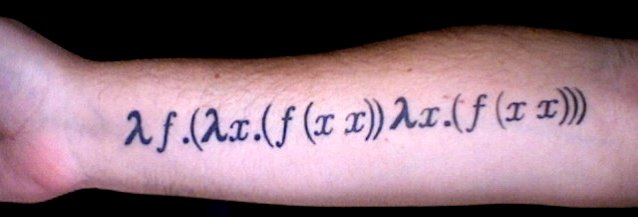
\includegraphics[height=4pc]{y-combinator.jpg}} \\
& = &  \lambda{f} . \bigl(\lambda{x} . f (x x)\bigr) \bigl(\lambda{x} . f (x x)\bigr)
\end{lcalc}

\begin{lcalc}
Y H & = & \Bigl(\lambda{f} . \bigl(\lambda{x} . f (x x)\bigr) \bigl(\lambda{x} . f (x x)\bigr)\Bigr) H \\
& \rightarrow & \bigl(\lambda{x} . H (x x)\bigr) \bigl(\lambda{x} . H (x x)\bigr) \\
& \rightarrow & H \Bigl(\bigl(\lambda{x} . H (x x)\bigr) \bigl(\lambda{x} . H (x x)\bigr)\Bigr) \\
& \leftrightarrow & H \biggl( \Bigl(\lambda{f} . \bigl(\lambda{x} . f (x x)\bigr) \bigl(\lambda{x} . f (x x)\bigr)\Bigr) H \biggr) \\
& = & H (Y H) \\
\end{lcalc}

``Y: The function that takes a function $f$ and returns $f(f(f(f(\cdots))))$''

\note{
\begin{enumerate}
\item It turns out we can define Y with a simple lambda expression!!!
\item Does anyone recognize the body of this lambda abstraction
(Answer: it's the expression that induced an infinite loop in our
discussion of normal form.)
\item To prove it, here we can see how Y H is equal to H (Y H). PROOF
(with penumltimate step due to beta-abstracting out H).
\item In essence, Y is the function that takes another function and
returns its potentially infinite sequence of applications. 
\item Applying the Y comb. to a single arugment usually doesn't
terminate; we get interesting, terminating functions when f takes two
or more arguments, like in factorial.
\end{enumerate}
}

\end{frame}

\begin{frame}[t]{Alonzo Church}

\vskip 1pc

  \begin{columns}
    \begin{column}{10pc}
      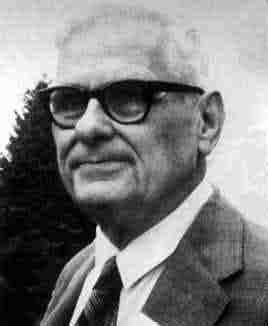
\includegraphics[height=6pc]{alonzo-church.jpg}
    \end{column}
    \begin{column}{15pc}

1903--1995

Professor at Princeton (1929--1967) \\
and UCLA (1967--1990)

Invented the Lambda Calculus

    \end{column}
  \end{columns}

Had a few successful graduate students, including

\begin{itemize}
\item Stephen Kleene (Regular expressions)
\item Michael O. Rabin$^{\dagger}$ (Nondeterministic automata)
\item Dana Scott$^{\dagger}$ (Formal programming language semantics)
\item Alan Turing (Turing machines)
\end{itemize}

$^{\dagger}$ Turing award winners

\note{
\begin{enumerate}
\item The guy who invented the lambda calculus is definitely a
theoretical CS legend.
\item His grad students weren't too shabby either.
\item In fact, his last grad student came up with his own
computational powerhouse...
\end{enumerate}
}

\end{frame}

\begin{frame}[t]{Turing Machines vs. Lambda Calculus}

\vskip 1pc

  \begin{columns}
    \begin{column}{10pc}
      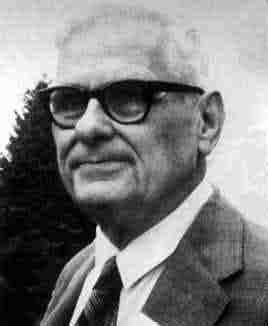
\includegraphics[height=6pc]{alonzo-church.jpg} \ \ 
      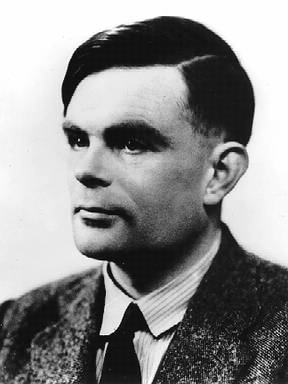
\includegraphics[height=6pc]{alan-turing.jpg}
    \end{column}
    \begin{column}{15pc}

In 1936,

\begin{itemize}
\item Alan Turing invented the Turing machine

\item Alonzo Church invented the lambda calculus
\end{itemize}

    \end{column}
  \end{columns}

In 1937, Turing proved that the two models were equivalent, i.e., that
they define the same class of computable functions.

Modern processors are just overblown Turing machines.

Functional languages are just the lambda calculus with a more
palatable syntax.

\note{
\begin{enumerate}
\item The TURING MACHINE!
\item Both the Turing machine and the lambda calculus were
independently developed in 1936. 
\item Then Turing bridged them together a year later -- equivalent!
\item These theoretical models form the underpinnings of many facets
of computer science.
\item Turing Machines -> processors
\item lambda-calc -> functional languages
\end{enumerate}
}

\end{frame}


\end{document}

% Local Variables:
% mode: latex
% compile-command: "make lambda.pdf"
% End:

